\documentclass[conference]{IEEEtran}
\usepackage[T1]{fontenc}
\usepackage[utf8]{inputenc}
\usepackage[brazil]{babel}
\usepackage{amsmath,amssymb}
\usepackage{booktabs}
\usepackage{graphicx}
\usepackage{cite}

\title{Otimização Multiobjetivo e Decisão no Caixeiro Viajante Biobjetivo}

\author{
\authorblockN{Cláudio Márcio Campos Paixão, Filipe Carvalho de Andrade e Matheus Cascalho dos Santos}
\authorblockA{Programa de Pós-Graduação em Engenharia Elétrica\\
Universidade Federal de Minas Gerais, Belo Horizonte, Brasil\\
EEE910A --- Otimização Multiobjetivo\\
Professor: Lucas S. Batista}
}

\begin{document}
\maketitle

\begin{abstract}
Este trabalho apresenta a terceira entrega do estudo do caixeiro viajante
biobjetivo com 250 cidades, cujos objetivos são minimizar tempo e distância.
O NeuroLKH foi executado em cinco repetições de 50 avaliações, totalizando
250 rotas. As cinco fronteiras aproximadas são comparadas e avaliadas em dez
momentos por repetição pelos indicadores hipervolume e $\Delta$, com pontos de
referência comuns estimados a partir da união das soluções. A frente global
não dominada contém oito alternativas. O AHP, aplicado a distância, tempo
nominal, emissão de CO$_2$ e Min-Max Regret, seleciona S6, com 18,5 h e
1.266,3 km. A razão de consistência dos julgamentos é 12,25\%, acima do limite
de referência de 10\%; por isso, a recomendação é provisória.
\end{abstract}

\section{Problema e instância}

O problema consiste em construir um circuito dirigido que parte da cidade 1,
visita cada uma das 250 cidades uma única vez e retorna à origem. Minimizam-se
simultaneamente o tempo total, em horas, e a distância total, em quilômetros,
somando os custos dos arcos da rota, inclusive o retorno. As matrizes de entrada
têm dimensão $250\times250$; a distância é simétrica e o tempo é assimétrico.
A formulação inteira e suas hipóteses foram apresentadas na primeira entrega
\cite{modelagem}.

As funções objetivo são conflitantes na amostra: o menor tempo observado,
17,9 h, ocorre em uma rota de 1.412,2 km, enquanto a menor distância,
1.204,4 km, requer 21,9 h. Portanto, uma única solução não minimiza ambos os
objetivos. Como o método empregado é heurístico, os resultados a seguir
representam aproximações e não certificam otimalidade global.

\section{Algoritmo e protocolo experimental}

O NeuroLKH combina uma Sparse Graph Network pré-treinada, que orienta a
seleção de arestas candidatas, com a busca local Lin--Kernighan--Helsgaun
(LKH) \cite{neurolkh}. Para explorar os dois objetivos, cada avaliação usa
uma escalarização dos custos normalizados,
$s_{ij}(w)=w\hat{t}_{ij}+(1-w)\hat{d}_{ij}$, variando o peso $w$ entre os
extremos do intervalo $[0,1]$. O LKH procura uma rota para cada peso; as rotas
são então avaliadas nas matrizes originais de tempo e distância.

A execução da instância de exemplo ``TSP BIOBJETIVO'' registra 50 iterações
por repetição, cinco repetições e semente
4180680559. Foram armazenadas 250 avaliações. Em cada repetição, a dominância
foi recalculada sobre as rotas daquela repetição, sem usar o rótulo de
dominância persistido para outra análise. As fronteiras resultantes contêm,
respectivamente, 3, 5, 4, 7 e 7 pontos. A união das cinco fronteiras, após
remover soluções dominadas globalmente, contém oito pontos distintos. A
Fig.~\ref{fig:repeticoes} sobrepõe as cinco fronteiras.

\begin{figure*}[t]
\centering
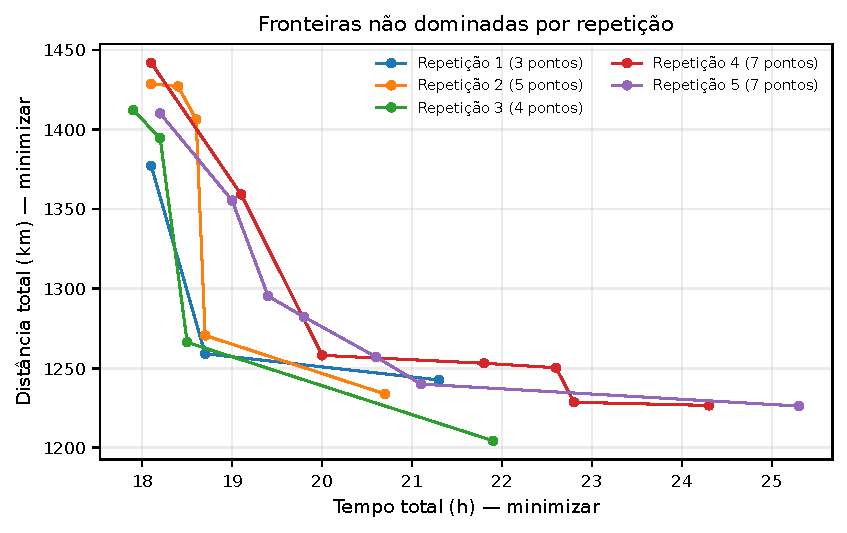
\includegraphics[width=0.76\textwidth]{figuras_entrega3/fronteiras_repeticoes.pdf}
\caption{Fronteiras não dominadas encontradas nas cinco repetições.}
\label{fig:repeticoes}
\end{figure*}

\section{Indicadores de qualidade}

\subsection{Referência comum e cálculo}

Como a fronteira Pareto ótima é desconhecida, os pontos de referência foram
estimados pela união das soluções não dominadas das cinco repetições. A
aproximação do ponto utópico é
$z^I=(17{,}9\ \mathrm{h},\,1.204{,}4\ \mathrm{km})$ e a do ponto
antiutópico (nadir) é
$z^N=(21{,}9\ \mathrm{h},\,1.412{,}2\ \mathrm{km})$. Cada objetivo foi
normalizado por
\begin{equation}
g_k(x)=\frac{f_k(x)-z^I_k}{z^N_k-z^I_k},\quad k\in\{t,d\}.
\end{equation}
Assim, o ponto de referência do hipervolume é $r=1{,}1z^N
=(24{,}09\ \mathrm{h},\,1.553{,}42\ \mathrm{km})$ nas unidades originais,
equivalente a $(1{,}5475,1{,}6796)$ no espaço normalizado. O valor reportado
é adimensional. O mesmo intervalo e o mesmo ponto de referência foram usados
nas cinco repetições e em todos os prefixos avaliados.

Para cada repetição, os indicadores foram calculados sobre a frente não
dominada do prefixo de $k=5,10,\ldots,50$ avaliações. O hipervolume
(S-metric) é a área da união dos retângulos entre cada ponto não dominado e
$r$:
\begin{equation}
HV(A)=\operatorname{area}\left(\bigcup_{g\in A}[g,r]\right).
\end{equation}
Geometricamente, mede a área dominada pela frente no espaço de objetivos.
Valores maiores indicam uma frente que cobre uma região maior, combinando
proximidade e extensão; o valor depende da normalização e do ponto de
referência \cite{zitzler}.

O indicador de espalhamento de Deb, $\Delta$, avalia a uniformidade do
espaçamento e a cobertura dos extremos \cite{deb}. Ordenando a frente por
tempo, sejam $d_i$ as distâncias euclidianas entre pontos consecutivos,
$\bar d$ sua média e $d^e_1,d^e_2$ as distâncias dos extremos observados aos
extremos de referência aproximados:
\begin{equation}
\Delta =
\frac{d^e_1+d^e_2+\sum_{i=1}^{|A|-1}|d_i-\bar d|}
{d^e_1+d^e_2+(|A|-1)\bar d}.
\end{equation}
Quanto menor $\Delta$, mais uniforme é o espaçamento e melhor a cobertura
dos extremos; zero representa espaçamento uniforme com cobertura perfeita.
Como não se conhece a frente exata, os extremos da união final servem de
aproximação comum. Ambos os indicadores foram recalculados nos dez prefixos
de cada repetição; as figuras mostram as cinco séries e sua média ponto a
ponto.

\subsection{Resultados}

O hipervolume médio sobe de 0,259 no quinto candidato para 2,029 no
quinquagésimo (desvio-padrão amostral final de 0,141), indicando aumento da
área coberta pela frente à medida que mais avaliações são incorporadas. O
espalhamento médio passa de 0,895 para
0,577; a trajetória não é monotônica, pois a inclusão de um novo ponto pode
alterar o espaçamento entre vizinhos. As curvas médias e a variação entre as
repetições são apresentadas nas Figs.~\ref{fig:hv} e \ref{fig:delta}.

\begin{figure}[t]
\centering
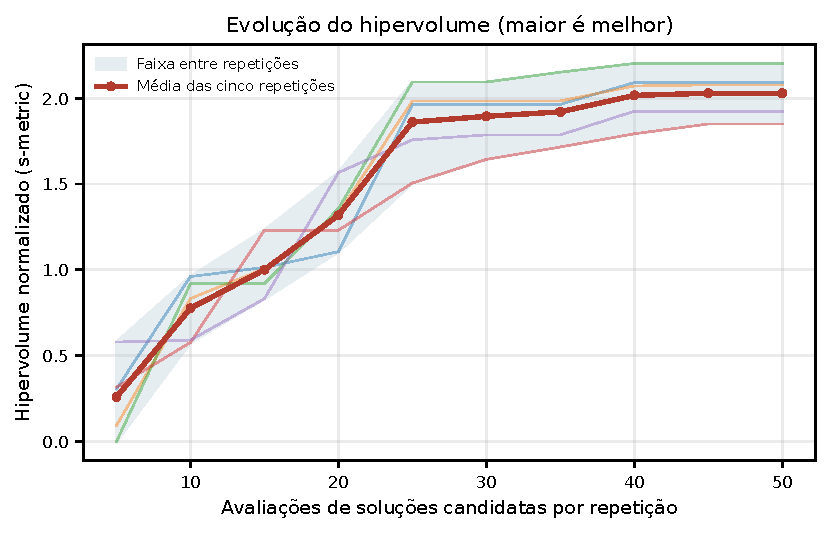
\includegraphics[width=\columnwidth]{figuras_entrega3/hipervolume.pdf}
\caption{Evolução do hipervolume em dez momentos. A linha destaca a média das cinco repetições.}
\label{fig:hv}
\end{figure}

\begin{figure}[t]
\centering
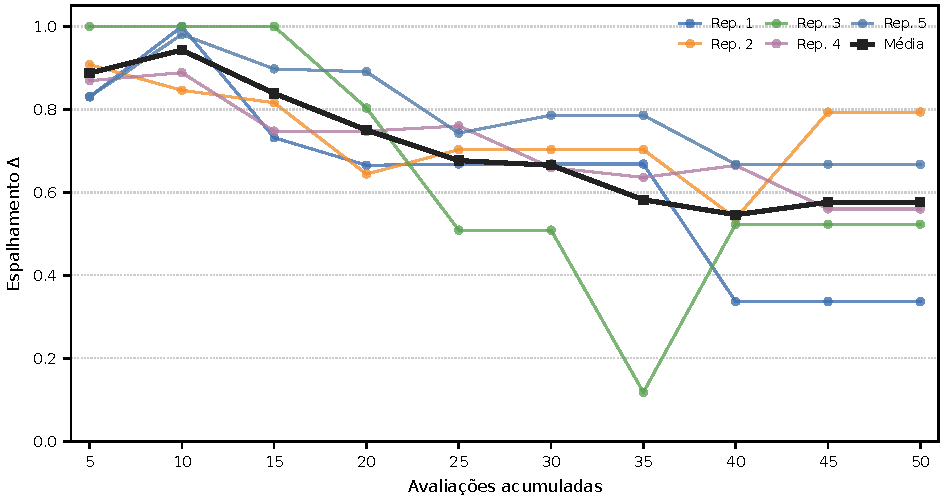
\includegraphics[width=\columnwidth]{figuras_entrega3/delta.pdf}
\caption{Evolução de $\Delta$ em dez momentos. Valores menores indicam melhor espalhamento.}
\label{fig:delta}
\end{figure}

\begin{table}[t]
\centering
\caption{Indicadores no 50\textsuperscript{o} candidato de cada repetição.}
\label{tab:indicadores}
\small
\begin{tabular}{crrr}
\toprule
Repetição & $|A|$ & $\Delta$ & $HV$\\
\midrule
1 & 3 & 0,290 & 2,091\\
2 & 5 & 0,792 & 2,077\\
3 & 4 & 0,528 & 2,202\\
4 & 7 & 0,537 & 1,850\\
5 & 7 & 0,738 & 1,924\\
\midrule
Média & --- & 0,577 & 2,029\\
\bottomrule
\end{tabular}
\end{table}

Há variação entre repetições: os hipervolumes finais vão de 1,850 a 2,202,
e $\Delta$ varia de 0,290 a 0,792. A repetição 1 tem o menor $\Delta$, mas
apenas três pontos; a repetição 4 tem sete pontos, mas o menor hipervolume.
Logo, quantidade de pontos não implica, por si só, melhor cobertura ou
espaçamento. A interpretação é relativa à amostra e às referências estimadas,
não uma comparação com uma frente ótima conhecida.

\section{Tomada de decisão multiatributo}

\subsection{Atributos e alternativas}

As oito alternativas da fronteira global foram mantidas na decisão, abaixo
do limite de 20 pontos. Além de distância e tempo nominal, foram considerados
dois atributos adicionais. A emissão estimada de CO$_2$ representa impacto
ambiental: para cada arco, calcula-se
$d_{ij}\cdot0{,}30\cdot q(v_{ij})$ kg, em que $v_{ij}=d_{ij}/t_{ij}$ e
$q$ vale 1,50 para velocidade inferior a 20 km/h, 1,15 de 20 a menos de
40 km/h, 1,00 de 40 a menos de 70 km/h e 1,20 a partir de 70 km/h. É uma
estimativa determinística, baseada nas matrizes da instância e no fator-base
assumido de 0,30 kg/km.

O Min-Max Regret mede a maior perda relativa da alternativa entre distância
e desempenho de tempo sob cenários simulados. O regret de distância é
$(d-d_{\min})/d_{\min}$; o regret temporal médio compara o tempo realizado
em cada cenário ao melhor tempo do conjunto e o normaliza pelo menor tempo
médio. A pontuação é o máximo entre esses dois regrets, portanto valores
menores são preferíveis. A análise usa 5.000 cenários Monte Carlo, semente
42, coeficiente de variação de 20\% nos tempos dos arcos e correlação
regional intra-arco de 30\%. Esses atributos não foram objetivos do
NeuroLKH; avaliam impacto ambiental e desempenho relativo sob incerteza.

\begin{table*}[t]
\centering
\caption{Alternativas não dominadas e ranking AHP. S6, em negrito, é a alternativa selecionada.}
\label{tab:alternativas}
\small
\begin{tabular}{crrrrrr}
\toprule
Rank & Solução & Distância (km) & Tempo (h) & CO$_2$ (kg) & Min-Max Regret & AHP (\%)\\
\midrule
1 & \textbf{S6} & \textbf{1.266,3} & \textbf{18,5} & 414,392 & 0,0514 & \textbf{17,284}\\
2 & S5 & 1.259,1 & 18,7 & 411,222 & 0,0479 & 17,193\\
3 & S7 & 1.377,2 & 18,1 & 456,573 & 0,1435 & 12,775\\
4 & S4 & 1.258,1 & 20,0 & 410,111 & 0,1204 & 12,700\\
5 & S8 & 1.412,2 & 17,9 & 469,668 & 0,1725 & 11,506\\
6 & S2 & 1.233,8 & 20,7 & 402,591 & 0,1597 & 10,741\\
7 & S3 & 1.257,1 & 20,6 & 412,299 & 0,1541 & 10,480\\
8 & S1 & 1.204,4 & 21,9 & 390,095 & 0,2267 & 7,320\\
\bottomrule
\end{tabular}
\end{table*}

\subsection{AHP e escolha}

O AHP foi aplicado em duas etapas \cite{saaty}. Os julgamentos par a par
dos critérios usam a escala de Saaty: distância/tempo $=1/9$,
distância/CO$_2=1/3$, distância/Min-Max $=1/5$, tempo/CO$_2=3$,
tempo/Min-Max $=1$ e CO$_2$/Min-Max $=2$; comparações não informadas são
neutras. Os pesos locais das alternativas são obtidos a partir de avaliações
monotônicas de desempenho em escala de 1 a 9, e a pontuação global é a soma
ponderada desses pesos locais.

\begin{table}[t]
\centering
\caption{Pesos dos critérios e consistência dos julgamentos.}
\label{tab:pesos}
\small
\begin{tabular}{lr}
\toprule
Critério & Peso\\
\midrule
Tempo nominal & 44,20\%\\
Min-Max Regret & 25,71\%\\
Emissão de CO$_2$ & 24,65\%\\
Distância & 5,44\%\\
\midrule
$\lambda_{\max}$ & 4,3308\\
Índice de consistência & 0,1103\\
Razão de consistência & 12,25\%\\
\bottomrule
\end{tabular}
\end{table}

S6 obtém 17,284\%, apenas 0,091 ponto percentual acima de S5. A preferência
forte pelo tempo nominal favorece S6 (18,5 h contra 18,7 h), embora S5 tenha
menor distância, menor emissão e menor Min-Max Regret. S1 ilustra outro
extremo: tem a menor distância e emissão, mas o maior tempo e regret; S8 tem
o menor tempo, mas maior distância e emissão. Esses compromissos explicam a
necessidade de ponderar os atributos, em vez de escolher pelo melhor valor
isolado.

A razão de consistência, 12,25\%, supera o limite de referência de 10\%.
Assim, o ranking é uma recomendação provisória: os julgamentos par a par
devem ser revistos, em especial porque a diferença entre S6 e S5 é pequena.
A probabilidade estimada de S6 pertencer à fronteira sob incerteza é 73,88\%;
seu tempo simulado médio é 18,5035 h e o CVaR$_{95}$ é 20,1620 h. Esses
resultados complementam a decisão, mas não eliminam a necessidade de rever
a consistência do AHP.

\begin{figure*}[t]
\centering
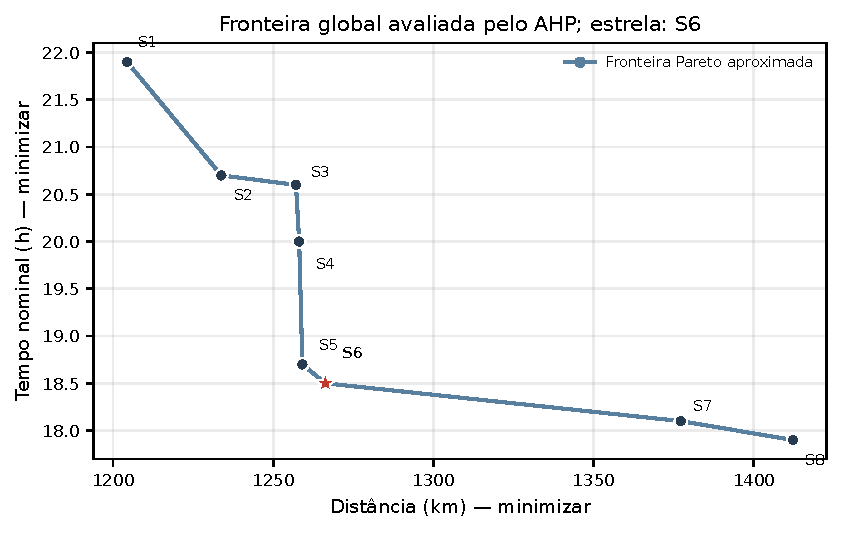
\includegraphics[width=0.76\textwidth]{figuras_entrega3/fronteira_decisao.pdf}
\caption{Fronteira global avaliada pelo AHP; a linha conecta os pontos e a estrela identifica S6. A distância está no eixo horizontal e o tempo no vertical.}
\label{fig:decisao}
\end{figure*}

\begin{figure}[t]
\centering
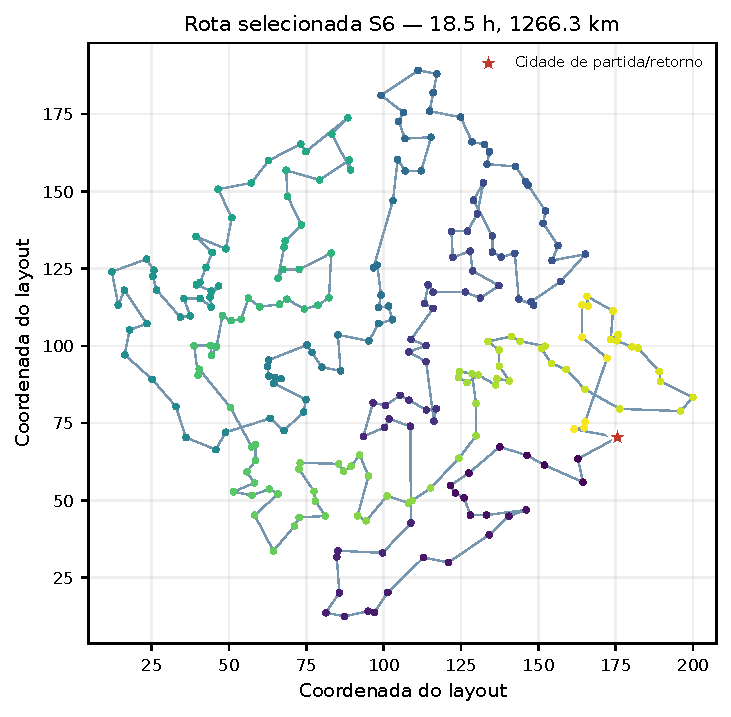
\includegraphics[width=0.88\columnwidth]{figuras_entrega3/rota_s6.pdf}
\caption{Circuito da alternativa S6: 250 cidades e retorno à cidade 1. As coordenadas representam o layout da instância, não um mapa geográfico.}
\label{fig:rota}
\end{figure}

\section{Conclusão}

Nas cinco repetições, o NeuroLKH produziu uma união global de oito soluções
não dominadas. A evolução média do hipervolume indica maior área coberta com
mais avaliações, enquanto $\Delta$ apresenta melhora média com variação entre
execuções. O AHP seleciona S6 pelo compromisso entre tempo nominal e os
atributos adicionais, mas sua vantagem sobre S5 é estreita. Como a razão de
consistência excede 10\%, a escolha deve ser considerada provisória até que
os julgamentos do decisor sejam revisados.

\begin{thebibliography}{00}
\bibitem{modelagem}
C. M. C. Paixão, F. C. de Andrade e M. C. dos Santos, ``Problema do
caixeiro viajante biobjetivo: modelagem inteira para minimização de tempo e
distância,'' EEE910A, Universidade Federal de Minas Gerais, 2026.

\bibitem{neurolkh}
L. Xin, W. Song, Z. Cao e J. Zhang, ``NeuroLKH: Combining deep learning model
with Lin-Kernighan-Helsgaun heuristic for solving the traveling salesman
problem,'' in \emph{Advances in Neural Information Processing Systems},
2021.

\bibitem{deb}
K. Deb, A. Pratap, S. Agarwal e T. Meyarivan, ``A fast and elitist
multiobjective genetic algorithm: NSGA-II,'' \emph{IEEE Transactions on
Evolutionary Computation}, vol. 6, no. 2, pp. 182--197, 2002.

\bibitem{zitzler}
E. Zitzler, M. Laumanns e L. Thiele, ``Comparison of multiobjective
evolutionary algorithms: Empirical results,'' \emph{Evolutionary
Computation}, vol. 8, no. 2, pp. 173--195, 2000.

\bibitem{saaty}
T. L. Saaty, \emph{The Analytic Hierarchy Process}. New York, NY, USA:
McGraw-Hill, 1980.
\end{thebibliography}

\end{document}
